%[Tamaño de letra, tipo de hoja, número de columnas]{tipo de documento}
\documentclass[12pt,letterpaper, onecolumn]{article}



%Decodificación para el lenguaje español y caracteres especiales.
\usepackage[utf8]{inputenc} 

%Definimos que trabajaremos en idioma español y el tipo de letra.
\usepackage[spanish]{babel}

%mejoras para mejorar la estructura de la información y la salida impresa de documentos que contienen fórmulas matemáticas.
\usepackage{amsmath}

%El paquete amsfonts brinda una colección de fuentes TeX adicionales diseñadas para su uso en material matemático con AmS-TeX.
\usepackage{amsfonts}

%El paquete amssymb permite usar símbolos especiales.
\usepackage{amssymb}

%Proporciona un índice ordenado a partir de datos sin procesar sin clasificar.
\usepackage{makeidx}

%El paquete se basa en el paquete de gráficos , proporcionando una interfaz clave-valor para argumenptos opcionales para el comando \ includegraphics .
\usepackage{graphicx}

%El paquete float es importante para las imágenes con la opción [H] para que las imágenes se coloquen en donde lo deseamos
\usepackage{float}

%A continuación vamos a definir los márgenes de nuestro documento con geometry
\usepackage[left=3cm,right=1.5cm,top=1.5cm,bottom=1.5cm]{geometry}

%Este paquete permite cambiar las formas de enumerar items.
\usepackage{enumerate}

%<<<<<<<<<<<<<<<<<<<<  >>>>>>>>>>>>>>>>>>>
%Agregaremos el siguiente paquete para cambiar el número de columnas (El menor número será el que definamos al inicio del documento)
\usepackage{multicol}

%\begin{multicols}{2}

%\end{multicols}
%<<<<<<<<<<<<<<<<<<<<  >>>>>>>>>>>>>>>>>>>

%A continuación veremos como podemos agregar un encabezado en nuestro documento:
%>>>>>>>>>>Forma para un solo autor
%\title{\LaTeX \hspace{0.1cm} en farmacia}
%\author{Departamento de química orgánica}
%\date{\today}

%>>>>>>>>>>Forma para varios autores

%Primero incluimos el paquete authblk: El paquete redefine el comando \ author para que funcione normalmente o para permitir un estilo de nota al pie de entrada de autor / afiliación.
\usepackage{authblk}


% El comando \ balance se puede utilizar para equilibrar las columnas en la página final si se desea. Debe colocarse en cualquier lugar dentro de la primera columna de la última página.
\usepackage{balance}

%\hspace es para espacio horizontales
\title{\LaTeX \hspace{0.1cm} en farmacia}


%[Número de afiliación]{Nombres, correos}
\author[2]{Gerson Alexander Cux García 
\thanks{gersoncux@ieee.org}}
\author[2]{Luis Armando Colorado Sequén \thanks{armando-colorado@ieee.org}}
\author[1]{Héctor Fernando Carrera Soto \thanks{hfcarrerasoto@ieee.org}}
\author[3]{Carmen Lucía Vásquez Maldonado \thanks{clvm.21@gmail.com}}
\author[3]{Federico Tzunux Tzoc
\thanks{fedetzunux10@gmail.com}}

%Agregamos afiliaciones y los enúmeramo [x]
\affil[1]{Universidad de San Carlos de Guatemala, Facultad de Ingeniería, IEEE-USAC RAS.}
\affil[2]{Universidad de San Carlos de Guatemala, Facultad de Ingeniería, IEEE-USAC EDS.}
\affil[3]{Universidad de San Carlos de Guatemala, Departamento de Química Orgánica.}
\affil[4]{Department of Mechanical Engineering, \LaTeX\ University}


%Con esto agregamos la fecha.
\date{\today}

%Paquete para configurar medidas de las tablas
\usepackage{tabularx}

%Para colocar hiperlinks \href{url}{text}
\usepackage[pdftex]{hyperref}

%<<<<<<<<< para saltos de página usar  \clearpage >>>>>
%<<<<<<<<< para saltos entre líneas usar \vspace{2cm}>>>>>

%<<<<<<<<< para espaciado horizontal \hspace{1cm}>>>>>

%<<<<<<<<< para colocar url o referencias a url usar \url{http://www.latex-project.org/} o  \href{http://www.latex-project.org/}{latex project}>>>>>>>


\begin{document}
%-----------------------------------------------------------------
%Antes de iniciar, debemos de indicar que los datos del título y autores, los vamos a ingresar.
\maketitle

%Colocaremos un índice.
\tableofcontents

%Explicar clear page, vspace y hspace
\clearpage
%\vspace{xcm}
%\hspace{xcm}
%-----------------------------------------------------------------
%Con \begin{abstract} indicamos que indicamos que inciaremos un resumen de nuestro trabajo.

\begin{abstract}
    Con el objetivo de sintetizar 6-fenil-2,7-dioxabiciclo[3.2.0]-3-hepteno a partir de ciclohexeno y 7-fenil-8-oxabiciclo[4.2.0]octano a partir de ácido furfurílico mediante una reacción de Paternó-Buchi, se mezclaron ambos sustratos con benzaldehído y se evaluó la reacción para ambos productos en diferentes condiciones. En la primera, se colocaron tubos (1 y 2) con los sustratos y benzaldehído en una cámara oscura con luz UV (390nm) y en la segunda, se colocaron tubos (3 y 4) con los sustratos y benzaldehído en otra cámara oscura con luz incandescente (100W). Se dejaron bajo las diferentes fuentes de energía por 24 horas y en ninguno de los casos se observó un cambio dentro del tubo de ensayo, por lo que se concluyó que la reacción no se había llevado a cabo.
\end{abstract}
%-----------------------------------------------------------------
%\section{} sirve para colocar
\section{Resultados}

%Colocando una tabla normal com tamaños definidos con tabular


%Colocando una tabla normal
\begin{table}[H]
\begin{center}
%\begin{tabularx}{\textwidth}{|m{0.10\linewidth}|m{0.20\linewidth}|m{0.20\linewidth}|m{0.20\linewidth}|m{0.20\linewidth}|}

\begin{tabular}{|p{1cm}|m{3cm}|m{3cm}|p{3cm}|p{3cm}|}
\hline 
	\textbf{No. de tubo} & \textbf{{Reactivos}
	contenidos
	en el tubo} & \textbf{Coloración y
	características de
	la mezcla antes de
	la reacción} & \textbf{Tipo y cantidad de
	fuentes de
	radiación utilizada} & \textbf{Coloración y
	características de
	la mezcla después
	de la reacción} \\ 
	\hline 
	1 & Ciclohexeno
	y
	benzaldehído & Incoloro y
	translúcido & 5 leds UV (5 mm y
	390 nm) & Incoloro y
	translúcido \\ 
	\hline 
	2 & Ácido
	furfurílico y
	benzaldehído & Color vinagre y
	translúcido & 5 leds UV (5 mm y
	390 nm) & Color vinagre y
	translúcido \\ 
	\hline 
	3 & Ciclohexeno
	y
	benzaldehído & Incoloro y
	translúcido & 1 foco
	incandescente (luz
	amarilla) 100 W & Incoloro y
	translúcido \\ 
	\hline 
	4 & Ácido
	furfurílico y
	benzaldehído & Color vinagre y
	translúcido & 1 foco
	incandescente (luz
	amarilla) 100 W & Color vinagre y
	translúcido \\ 
	\hline 
	\end{tabular} 
\caption{Aspectos cualitativos antes y después de la reacción.}
\centering{Fuente: Datos experimentales obtenidos en el Laboratorio 01, Departamento de Química Orgánica, edificio T12.
USAC.}
\label{Tab_Colocando_una_tabla}
\end{center}
\end{table}

%Explicar subsection
\subsection{Parámetros para colocar tablas}



\begin{table}[H]
\begin{center}
    %Explicar como funciona p, m y c.
	\begin{tabular}{|p{3cm}|m{3cm}|b{3cm}|c|}
	\hline 
	p & m & b & c \\ 
	\hline 
	texto que es considerablemente más largo que el ancho de la columna & 
	texto que es considerablemente más largo que el ancho de la columna & 
	texto que es considerablemente más largo que el ancho de la columna & 
	texto que es considerablemente más largo que el ancho de la columna \\ 
	\hline 
	\end{tabular} 
\caption{Formas de alineación.}
%Aquí \url nos sirve para colocar un enlace, también podemos usar \href{http://www.latex-project.org/}{latex project}
\centering{Fuente: \url{https://n9.cl/zlsb7}}
\label{Tab_Parámetros_1}
\end{center}
\end{table}


%Explicar como colocar la tabla en donde la queremos
\begin{table}[H] 
\begin{center}
	\begin{tabular}{|m{2cm}|m{2cm}|m{2cm}|m{2cm}|m{2cm}|m{2cm}|}
	\hline 
	\textbf{h} & \textbf{t} & \textbf{b} & \textbf{p} & \textbf{!} & \textbf{H} \\ 
	\hline 
	Colocará la tabla aquí aproximadamente. & Coloque la tabla en la parte superior de la página. & Coloque la tabla en la parte inferior de la página. & Ponga la tabla en una página especial, solo para mesas. & Anula los parámetros internos de \LaTeX & Coloque la tabla en esta ubicación precisa, casi como h !. \\ 
	\hline 
	\end{tabular} 
\caption{Parámetros para fijar una tabla.}
\centering{Fuente: \url{https://n9.cl/sgzc4}}
\label{Tab_fijar_una_tabla}
\end{center}
\end{table}

%Explicar como quitar enumeración de las secciónes y otros.
\subsection*{Probando no enumerar esta subsección}

\begin{table}[H]
\begin{center}
    %Explicar como funciona p, m y c.
    \begin{tabular}{|c|c|c|}
    \hline 
    \textbf{Imagen 1} & \textbf{Imagen 2} & \textbf{Imagen 3} \\ 
    \hline 
    
\includegraphics[scale=0.09]{IEEE.png} & 
\includegraphics[width=3cm,height=1.65cm]{IEEE_RAS_logo-2.png} & 
\includegraphics[scale=0.45]{EDS_LOGO.jpg} \\ 
    \hline 
    \end{tabular} 
\caption{Formas de alineación.}
%Aquí \url nos sirve para colocar un enlace, también podemos usar \href{http://www.latex-project.org/}{latex project}
\centering{Fuente: \url{https://www.ieee.org}}
\label{Tab_imágenes_en_una_tabla}
\end{center}
\end{table}

%------------------------------------------------------
\section{Ecuaciones: ejemplos}

Para insertar ecuaciones dentro de un texto, se puede hacer de 2 formas : $ y=ax^2+bx+c $. y \( y=ax^2+bx+c \).
\\
\begin{equation}
    f(x)=ax^2+bx+c
\end{equation}

\begin{equation}
    f(x)=mb+x
    \label{Ec_recta}
\end{equation}

\begin{align}
    f(x)=x^3+1 \\
    g(x)=2x \\
    f(x)+g(x)=x^3+2x+1
\end{align}


\begin{align}
    \tag{1.1} f(x) &=x^3+1   & w &=y \\
    \tag{1.2} g(x) &=2x & z &=x+y\\
    \tag{A}   f(x)+g(x) &=x^3+2x+1
\end{align}

\textbf{Forma 1 para quitar la numeración (Corta)}

\begin{align*}
    f(x) &=x^3+1    & w &=y  & z=1\\
    g(x) &=2x       & z &=x+y\\
    f(x)+g(x) &=x^3+2x+1
\end{align*}

\textbf{Forma 2 para quitar numeración (Larga)}

$$ y= x^3+x^2+5x+2 $$

$$ y= x^3+5x+2 $$


\subsection{Fracciones}

Insertar fraciones $ 3/5 = \frac{3}{5} = \dfrac{3}{5} = \tfrac{3}{5} = \cfrac{3}{5} $


$$ 3/5 = \frac{3}{5} = \dfrac{3}{5} = \tfrac{3}{5} = \cfrac{3}{5} $$

$$ \dfrac{ 1+\dfrac{x+1}{x-2} } {\dfrac{x-2}{x+1}+\dfrac{3x}{2}} $$

$$ \frac{ 1+\frac{x+1}{x-2} } {\frac{x-2}{x+1}+\frac{3x}{2}} $$

\subsection{Raíces y Exponentes}

$$ \sqrt{x+y+12} $$

\begin{align*}
    z &= \sqrt{x+y+12} \\
    z &= \sqrt{ \dfrac{2x+1}{2x+1} } \\
    z &= \dfrac{ \sqrt{2x+1}}{2x+1} \\
    z &= (x+1)^{1/3} = \sqrt[7]{x+1}
\end{align*}

Superindice

$$ y=mx^{2x}+b $$

Subindice

$$ Y=mx_{prima}+b$$


\subsection{Signos de Agrupación}

\begin{align*}
    z &=x^3+y^3 \\
    z &= (x+y)(x^2-xy+y^2) \\
    z &= (\dfrac{2x}{y})^2 & [\dfrac{2x}{y}]^2 \\
    z &= \left (\dfrac{2x}{y} \right)^2 \\
    z &= \left [\dfrac{2x}{y} \right]^2 \\
    z &= \left \{ \dfrac{2x}{y} \right \}^2 \\
    z &= \left< \dfrac{2x}{y} \right> ^2
\end{align*}



%-----------------------------------------------------------------
\begin{multicols}{2}

\section{Análisis de resultados}

La   reacción   Paternó-Büchi   se   basa   en hacer   reaccionar   el doble   enlace   de   un grupo  carbonilo  con  un  alqueno  mediante excitación  fotoquímica.  Los  productos  de esta   reacción   poseen un   núcleo   de oxetano   (ver  mecanismo  de  reacción  en anexo   2).   El   carbonilo   reacciona   al obtener  su  estado  triplete. Para  que  esto suceda,   la   fuente   de   radiación   debe excitar el   par   electrónico   del   enlace $\pi$ oxígeno-carbono  a  un  estado  singlete  (los espines   del   par   electrónico   son antiparalelos),  luego,  este  estado  decae  al estado  triplete  que es  menos  energético  y en  el  cual  los  espines  de  los  electrones  de este   enlace   $\pi$  son   paralelos   (Levine, 2004; Li, 2014)
\\

Como  se  puede  observar  en  la  tabla  No.1,  no  existieron cambios  en  la  mezcla  de las   reacciones  1  y  2  luego  de  24  horas bajo  la  fuentes  de  energía.  Esto  se  pudo deber  a  que tal  y  como  ya  se  mencionó  en el  párrafo  anterior  el carbonilo reacciona al   estar   en   su   estado   triplete  lo  que  se consigue  con  radiación  UV.  Sin  embargo, la  luz  en  las  longitudes  de  onda  UV  son absorbidas  por  el  vidrio,  que  es  el  material del  que  están  hechos  los  tubos  de  ensayo utilizados  como  recipientes  de  contención de   las   distintas   soluciones,   como   se puede  ver  en  el  anexo  4.  Este  hecho  pudo causar  que  el  benzaldehído  no  absorbiera la  radiación necesaria  para  que  se  llevara a   cabo   la   reacción   (Skoog   et  al., 2008).
\\

Por   otro   lado,   en   los   tubos   3   y   4   (ver anexo  5),  tampoco  se  observó  cambio  en las   características   de   las   soluciones contenidas   en  los  mismos  (tabla  No.  1). Esto   pudo ser   a   que   los   reactivos utilizados  pudieron  volatilizarse  ya  que  el parafilm   usado   para   evitar   esto,   fue            
deshecho   por   el   calor   producido   con  el  foco incandescente  y  ser  causa  de  que  no existiera   reacción   (Boylestad, 2004). 
\\

Se   esperaba   que   al   realizar   una caracterización  comparando los  espectros infrarrojos   de   los   productos   con   el   del benzaldehído  (ver  anexo  3),  estos  ya  no presentarán   las   bandas   a   2820,  2756  y 1703   cm -1 ,   pues   son   las   bandas características   del  carbonilo  presente  en el   benzaldehído (Wade,   2011).  Esto  es debido  a  que  como  se  puede  observar  en el  anexo  2,  es  este  grupo  el  que  reacciona con   el   doble enlace   para   formar   el heterociclo   de   cuatro   miembros   que se espera  en  el  producto  (Thompson,  et  al., 2015).  Sin  embargo,  como  la  reacción  no se  llevó  a  cabo,  se  hubiera  obtenido  un espectro  con  una  mezcla  de  los  picos  del benzaldehído  con  los  del  sustrato  o  solo del   benzaldehído   en el   caso   que   los sustratos   se   hayan   evaporado.  

\section{Conclusiones}

\begin{itemize}
    \item La   falta de diferencias en las características   de   las soluciones de   los   cuatro   tubos   al  inicio  y  al final del tiempo  en  el  que se encontraron   bajo   las   fuentes de radiación  indicaron  que  no  existió reacción   en   ninguno   de estos. 
    \item Se determinó que una causa por la cual no existió reacción en los tubos de 1 y 2 es que se utilizaron tubos de vidrio ya que es u material que absorbe la luz UV.
    \item El motivo por el cual las reacciones de los tubos 3 y 4 no tuvieron lugar, fue la volatilización de los sustratos debido a la pérdida del parafilm utilizado para tapar los tubos.
    \item Debido a que la reacción no se llevó a cabo, en el espectro IR de los productos se podrían observar las bandas características del carbonilo del benzaldehido.
\end{itemize}

\section{Recomendaciones}

\begin{itemize}
    \item Colocar las luces led dentro del tubo de ensayo para que la radiación pase directamente a los sustratos y no sea absorbida por el vidrio (Skoog, et al., 2008).
    \item Tapar los tubos de ensayo que se van a colocar en la luz incandescente con algún material que no se deshaga o descomponga tan fácilmente con el calor (Boylestad, 2004), como por ejemplo un corcho.
\end{itemize}

\end{multicols}
\balance
%-----------------------------------------------------------------
%-----------------------------------------------------------------
\section{Anexos}

\begin{figure}[H]
    \centering
    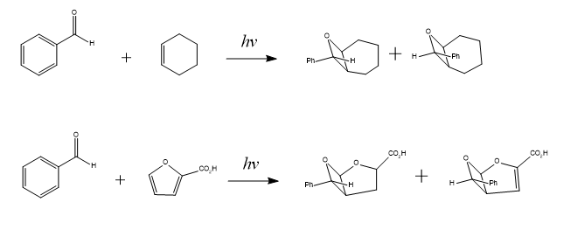
\includegraphics[scale=0.75]{Anexo_1.png}
    \caption{}
    \centering{Fuente: Thompson et al, 2015; Li, 2014 }
    \label{Fig_1}
\end{figure}


\begin{figure}[H]
    \centering
    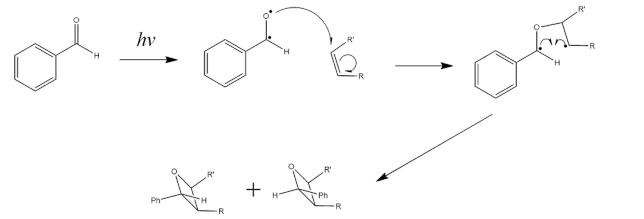
\includegraphics[scale=0.75]{Anexo_2.png}
    \caption{Mecanismo general de las reacciones realizadas}
    \centering{Fuente: }
    \label{Fig_2}
\end{figure}

%Aquí explicamos el comando [width = \columnwidth]

\begin{figure}[H]
    \centering
    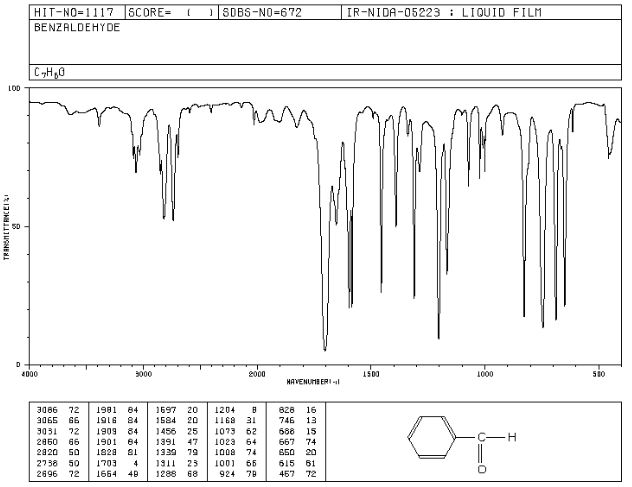
\includegraphics[width = \columnwidth]{Anexo_3.png}
    \caption{}
    \centering{Fuente: Spectral Database for Organic Compounds, 2019.}
    \label{Fig_3}
\end{figure}


\newpage

\\
%-----------------------------------------------------------------
%-----------------------------------------------------------------
\begin{multicols}{2}

\section{Anotaciones de pié de página y referencias}

\begin{enumerate}
    \item footnote \{ \}
    
    \item ref \{ \}
    
    \item cite \{ \}
    
    \item url \{URL\}
    
    \item href \{URL\}\{Texto mostrado\}
\end{enumerate}

Probaremos los comandos antes descritos.\\

\begin{enumerate}[I)]
    \item \textbf{footnote:} Lo usamos para hacer notas al pié de página\footnote{Usando footnote.}.
    
    \item \textbf{ref:} Lo usamos para hacer referencias de cuadros, imágenes y ecuaciónes. Ejemplo de una referencia de la tabla \ref{Tab_Colocando_una_tabla}, figura \ref{Fig_2} y ecuación \ref{Ec_recta}.
    
    \item \textbf{cite:} Lo usamos para hacer referencias bibliográficas, pero debémos agregarles etiquetas a las referencias ''bibitem{etiqueta}''. Haciendo de la siguiente subsección, \textbf{''Historia del IEEE''} \cite{biblio_4}.
    
    \item \url{https://usac.ieee.org.gt/}
    
    \item \href{https://usac.ieee.org.gt/}{Enlace a la página oficial del IEEE USAC \textbf{(Click aquí)}.}
    
\end{enumerate}

\subsection{Historia del IEEE}
El Instituto de Ingenieros Eléctricos y Electrónicos (IEEE\footnote{El IEEE es una institución a nivel global, la cuál está dividida por regiónes.}, Institute of Electrical and Electronics Engineers), es la mayor organización profesional técnica del mundo, que agrupa a más de  420.000 ingenieros, científicos, tecnólogos y profesionales en más de 160 países, que se dedican al avance en la innovación tecnológica y a la excelencia en beneficio de la humanidad.\\

IEEE, nació el 1 de enero de 1963 con la fusión de dos organizaciones previas, el American Institute of Electrical Engineers (AIEE), fundada en 1884 por Thomas A. Edison y Alexander G. Bell, entre otros, y el Institute of Radio Engineers (IRE), fundada en 1912. Por este motivo las actividades iniciales del IEEE cubrían temas relacionados con la ingeniería eléctrica y las comunicaciones, pero, en la actualidad, el IEEE cubre un espectro tecnológico mucho más amplio: desde la nanotecnología, hasta la ingeniería oceánica, pasando por bioingeniería, robótica, electromagnetismo, fotónica, procesado de señal, electrónica y ciencia de ordenadores, por citar unas pocas áreas.\\

\subsection{El IEEE en la actualidad}

Los miembros más importantes dentro del IEEE son los estudiantes, ya que constituyen el futuro de la organización. En estos momentos casi el 25\% del total de miembros del IEEE pertenecen a este sector y su implicación en las actividades de la Sección es muy elevada. Los estudiantes de una misma universidad se agrupan formando una Rama de Estudiantes (Student Branch-SB), para organizar distintos tipos de eventos científico-técnicos, de formación, visitas a instalaciones singulares y otras actividades complementarias.\\

Las publicaciones de IEEE son una de las fuentes de información técnica más importantes para científicos e ingenieros de todo el mundo en un gran número de ramas. En particular estas publicaciones constituyen alrededor del 30\% de las publicaciones técnicas en los campos de la ingeniería eléctrica, la electrónica y la informática.\\

IEEE promociona anualmente más de 1800 conferencias internacionales alrededor del mundo, en todas las áreas de interés de sus Sociedades.\\

Finalmente, IEEE es el líder en el desarrollo de estándares para la industria, con más de 1300 estándares activos (y 600 más en desarrollo), entre los que destaca el estándar wifi, IEEE 802.11. Está información se encuentra disponible para todo el público\cite{biblio_4}.\\


%-----------------------------------------------------------------
\begin{thebibliography}{99}
%Las fuentes de consulta se citan en forma organizada y homogénea, tanto de los libros, de los artículos y, en general, de las obras consultadas, que fueron indispensables indicar o referir en el contenido del trabajo.

\bibitem{biblio_1} Boylestad, R. (2004). \textit{Introduccion al análisis de circuitos.}. Pearson Education.

\bibitem{biblio_2} Levine, I. (2004). \textit{Name Reactions: A Collection of Detailed Mechanisms and Synthetic Applications. Springer.}.

\bibitem{biblio_3}Skoog, D., West, D., Holler, F. y Crouch, S.  (2008). \textit{Principios de Análisis Instrumental.}. Mexico: Cengage Learning

\bibitem{biblio_4} Quienes Somos. (s.f.). IEEE Sección España. Recuperado 29 de septiembre de 2021, de :\\
\url{https://ieeespain.org/quienes-somos/}

\bibitem{Original} Tzoc, F., Alva, R., Betancourth, A., \& Lemus, C. (2020). Tarea laboratorio teórico RMN 1. 6. \%(s.f.) = Sin fecha

\end{thebibliography}

\end{multicols}
\balance

\end{document}